\subsection{Multi-version} \label{multi}

Multi-version techniques build on the idea of multiple software versions which all meet the same specifications. These versions are interchangeable in terms of their output, but each version executes differently from the rest, ensuring that no two version share the same resources.
Multiple versions of the same software are executed either in sequence or in parallel, each utilizing different error detection and recovery methods, to have the highest probability of completing the task successfully.

\subsubsection{Recovery blocks}

Recovery blocks is a simple form of multi-version programming, expanding upon the idea of "checkpoint and restart". Unlike its single version counterpart, however, recovery blocks does not re-execute the same code again, but instead chooses a different version to try next.

A key advantage of the recovery blocks technique is that, in most cases, the primary version will be the only one to execute \cite{lyu:sft}, allowing alternate versions to prioritize redundancy and safety over performance. This enables the design of backup versions with gradually reduced performance requirements, ensuring robust fallback options without excessive resource consumption.

% \begin{figure}[hbt!]
%     \centering
%     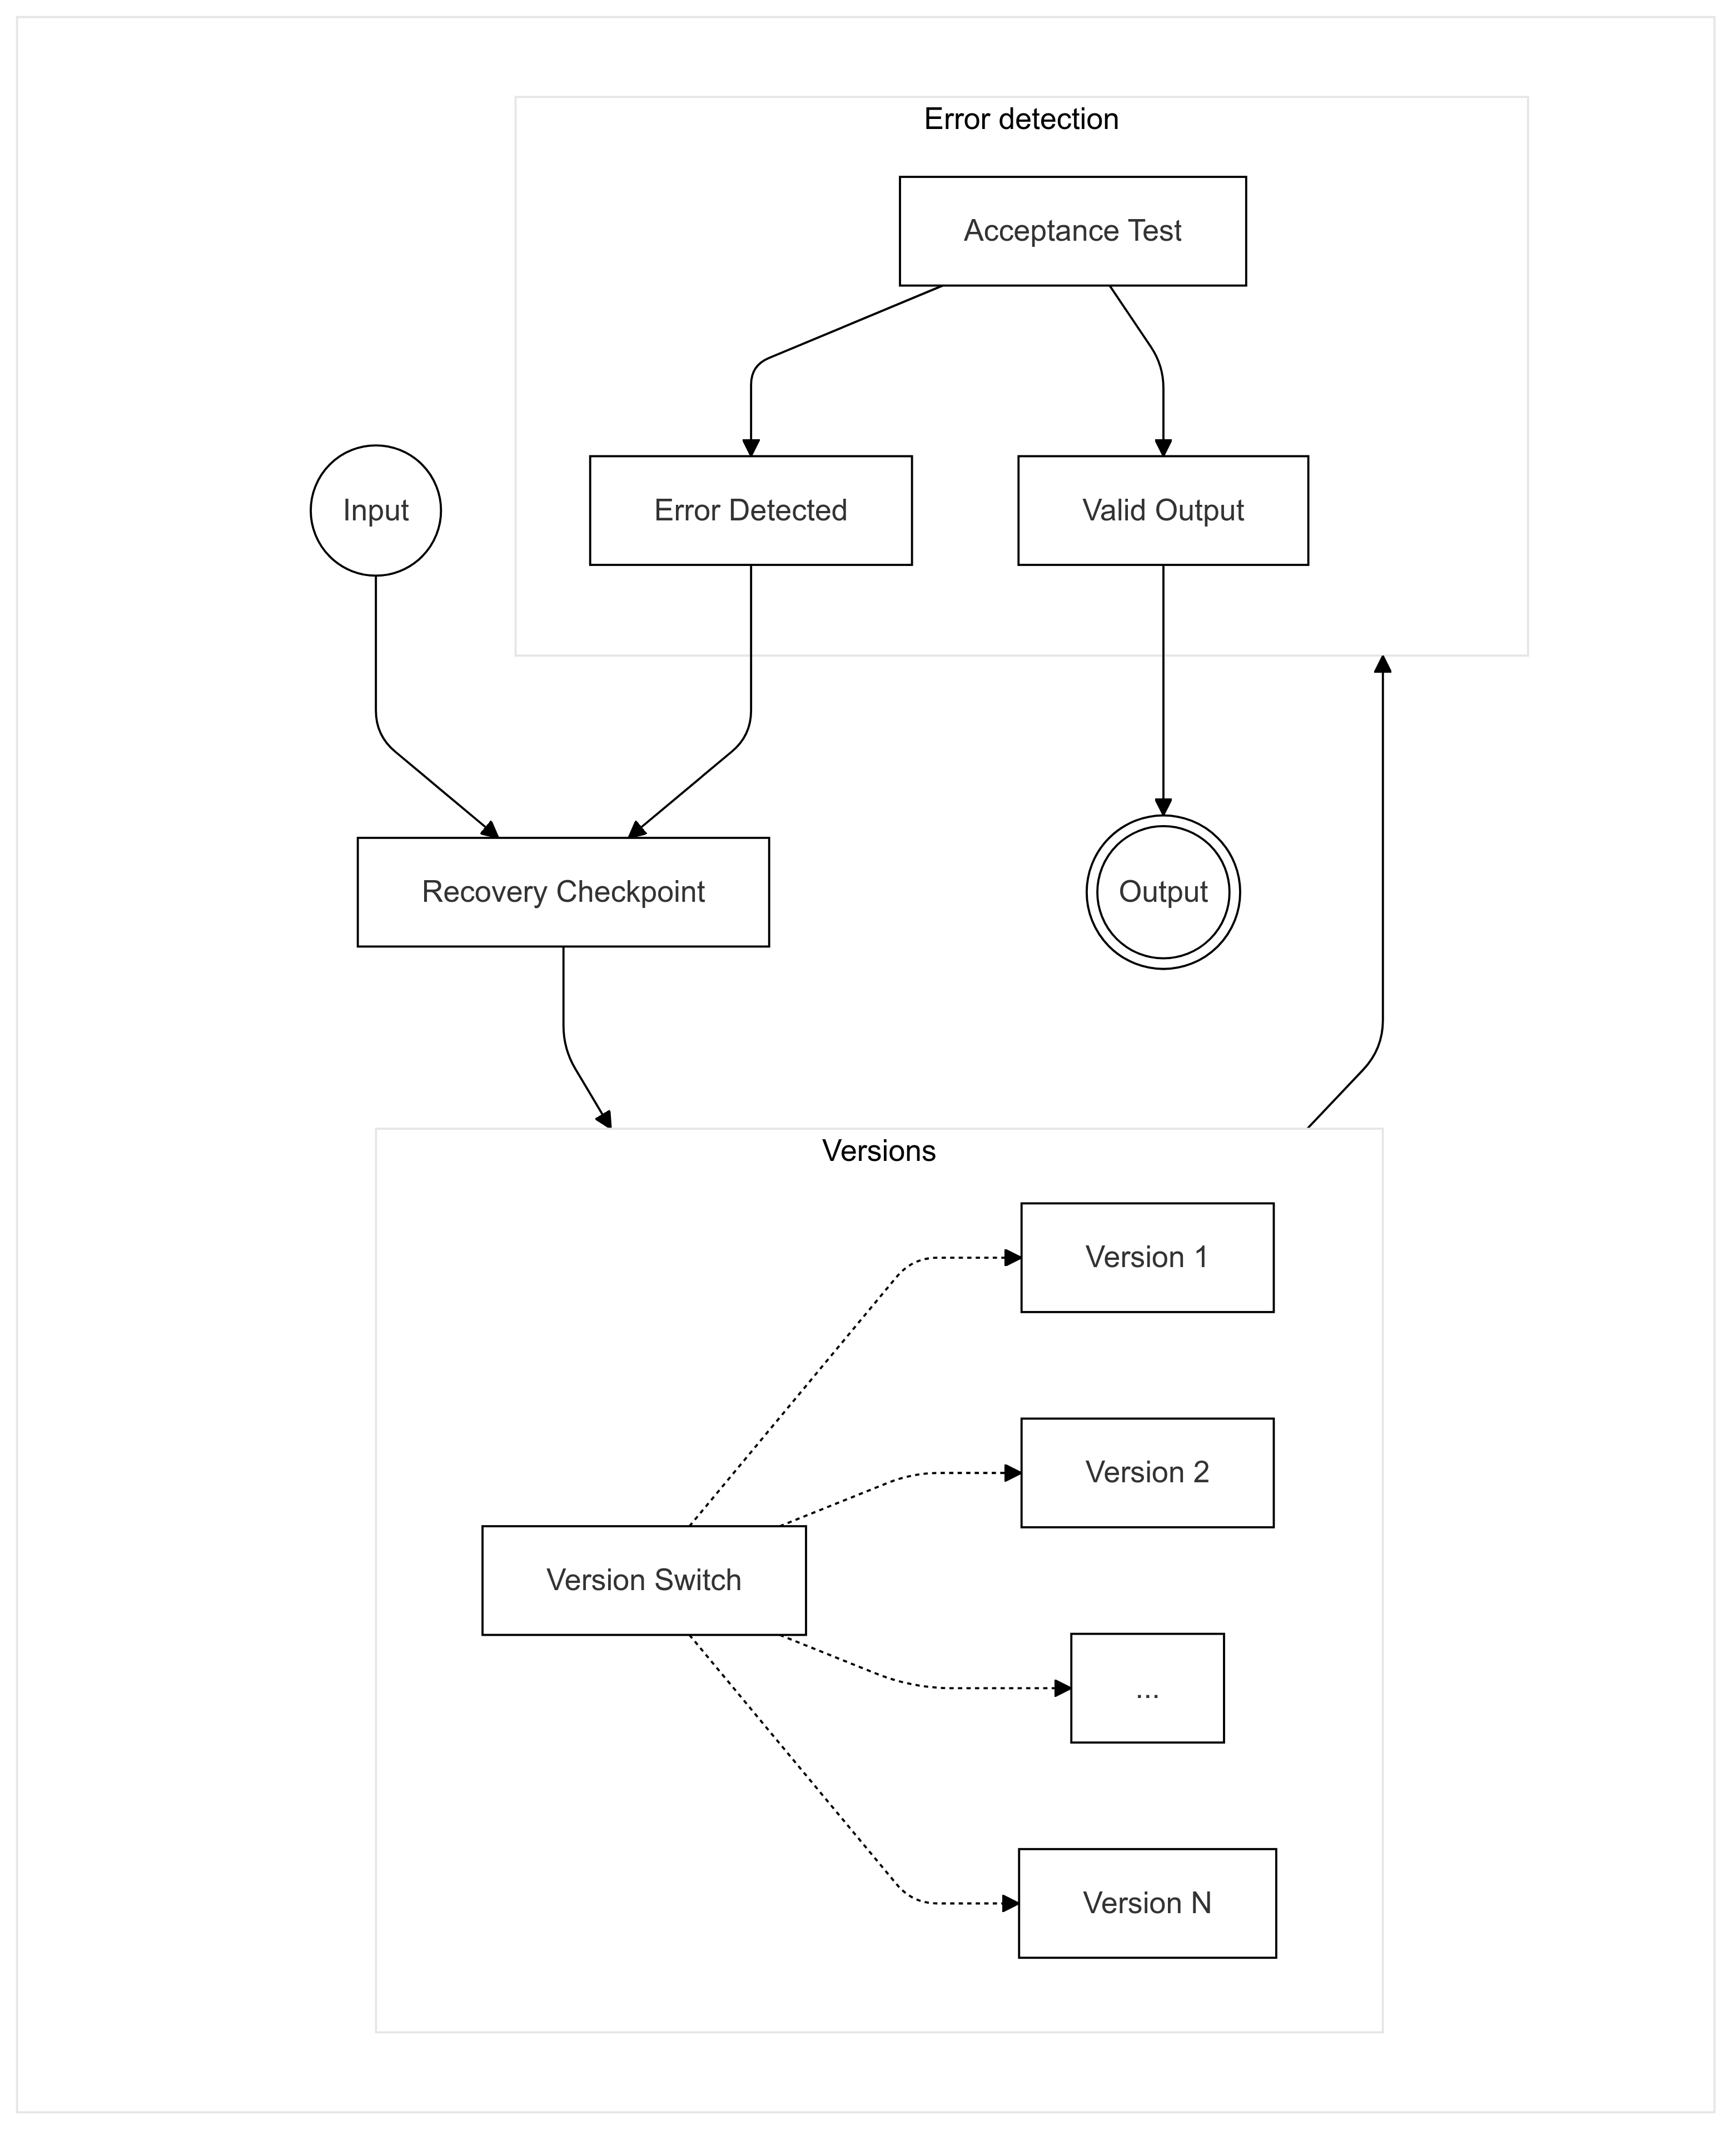
\includegraphics[width=0.9\textwidth]{recovery_blocks/recovery_blocks_01.png}
%     \caption{Recovery Blocks}
%     \label{fig:rec_blo}
% \end{figure}

% \break

Since faults are relatively rare compared to normal execution, this approach often achieves an optimal balance of performance and reliability. In some situations, the alternate versions do not necessarily have to produce a correct result, but a result that satisfies the acceptance check \cite{lyu:sft}. Alternate version can gradually degrade the service in order to accomplish the bare minimum requirements.

The overall success of the recovery block scheme rests to a great extent on the effectiveness of the error detection mechanisms used — especially (but not solely) the acceptance test. The acceptance test must be simple otherwise there will be a significant chance that it will itself contain design faults, and so fail to detect some errors, and/or falsely identify some conditions as being erroneous. Moreover, the test will introduce a run-time overhead which could be unacceptable if it is very complex. The development of simple, effective acceptance tests can thus be a difficult task, depending on the actual specification \cite{lyu:sft}.

A considerable drawback of recovery blocks is its inability to detect faults which might appear as normal execution of the program. As an example, if a bit-flip in the output register of a function results in a value that the acceptance check does not consider invalid an incorrect result will be returned. This error would go undetected without additional checks on top of recovery blocks.

\subsubsection{N-version programming}

\Acrfull{nvp} \cite{aa:nvp} extends the multi-version technique by running "N" independent versions in parallel or in sequence, hence “N-version” programming. In this approach, each version meeting the same specifications independently performs the task, and the final outcome is determined through a consensus mechanism that evaluates the results from all N executions.

This consensus is usually achieved through a voting algorithm, which aggregates the outputs from each version and selects the result agreed upon by the majority. Selection algorithms are an entire topic of its own covered well by \cite{Aljarbouh_2021}.

This voting approach to handling errors is sometimes referred to as \textbf{fault masking}, since we are not necessarily concerned with detecting an error, but rather getting an acceptable output even in the presence of a fault.

\begin{figure}[hbt!]
    \centering
    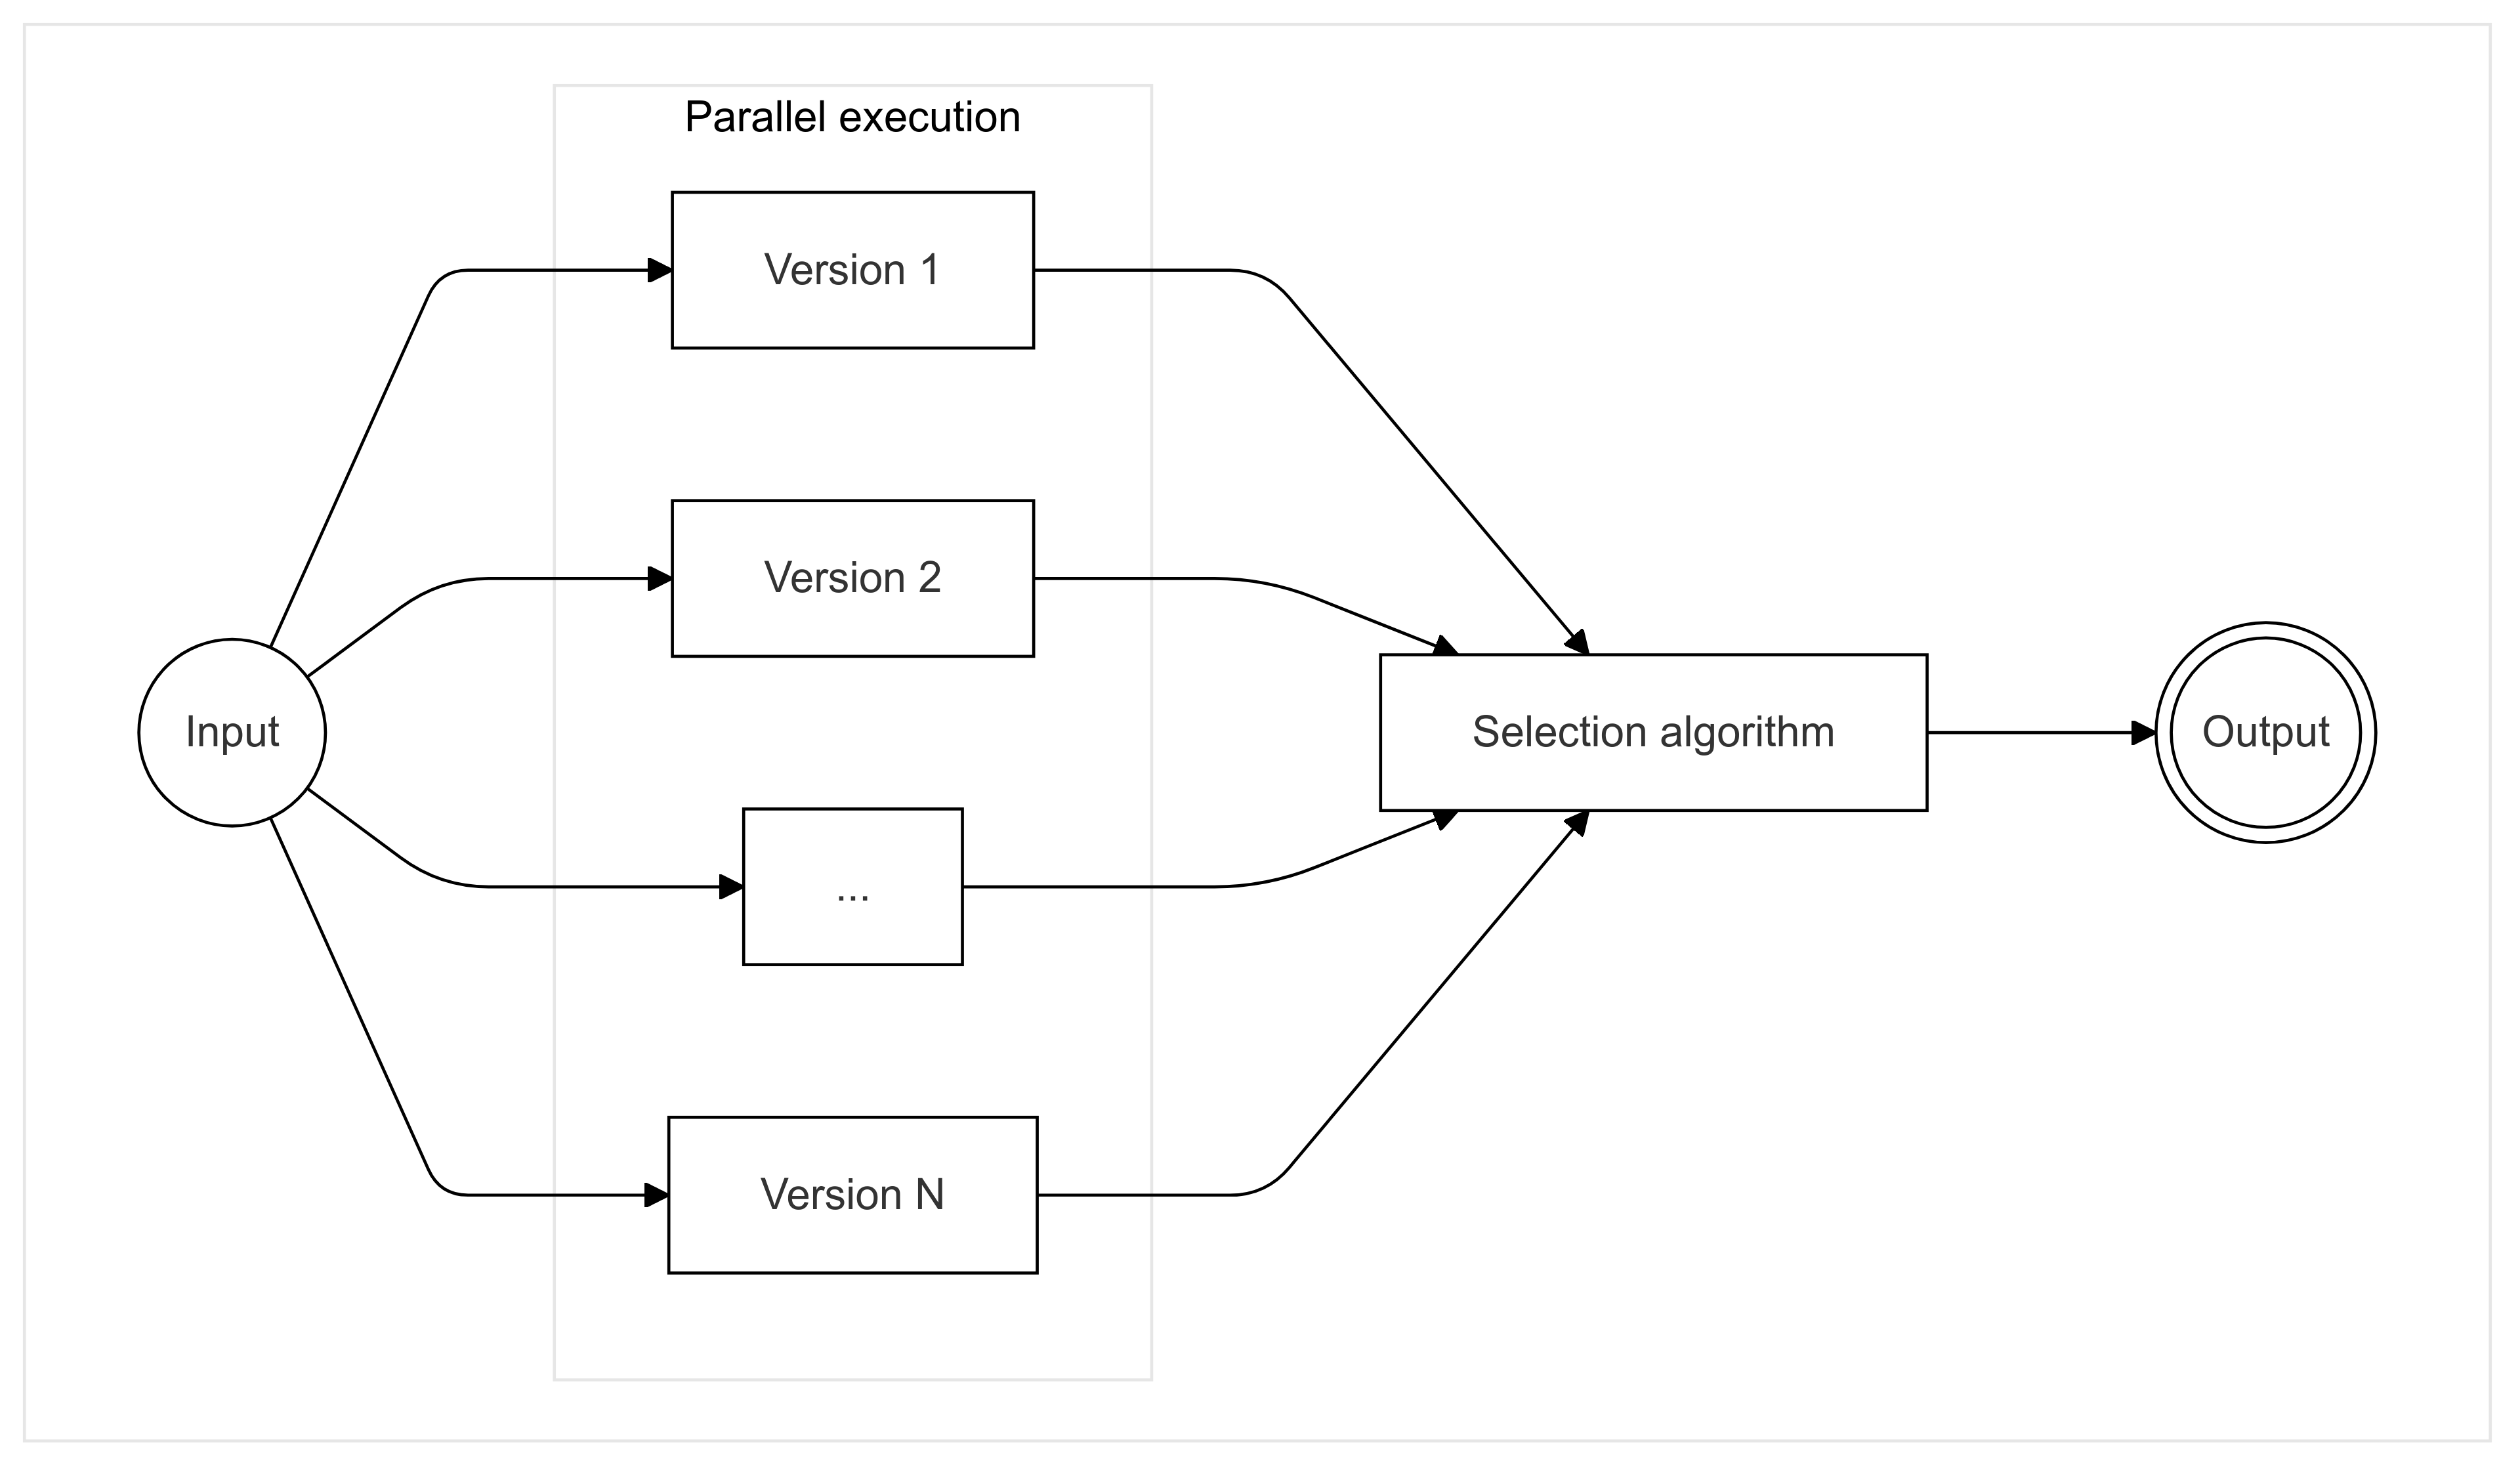
\includegraphics[width=0.9\textwidth]{n_version_prog/n_version_prog.png}
    \caption{N-Version Programming}
\end{figure}

The primary drawback of \acrshort{nvp} is its requirement to execute all of the versions before determining the final output. This can be highly resource-intensive, especially for large or complex tasks, as it requires significant computational power and memory to run multiple versions simultaneously.

For systems with limited resources, such as embedded systems, this approach can be particularly inefficient. The need to allocate resources for each version can strain the system's capabilities, potentially reducing its overall performance and responsiveness. As a result, while \acrshort{nvp} enhances fault tolerance and reliability, it may not be suitable for applications where resource constraints are a priority or where processing efficiency is critical.

A consideration for \acrshort{nvp} is the possibility of an error not being a random event, but rather a function of the input variables \cite{5326}. Therefore, even multiple versions running in parallel could all fail and give erroneous results. This makes the selection algorithm a critical failure point which \acrshort{nvp} on its own does not address.

\subsubsection{N Self-checking programming}

\Acrfull{nscp} \cite{nscp} is an extension of the classic \acrshort{nvp}, where on top of executing multiple versions, each version also contains its own independent acceptance test or recovery block, before the results are passed to the selection logic. The selection logic then selects the "topmost" possible version that reports a correct output.

A version-specialized acceptance check is an interesting addition, as it provides the opportunity to take advantage of the version implementation details. We can specifically tailor the check to consider the inner workings of the version to detect errors and possibly even correct them before proceeding to the selection stage.

The drawback here is the increase in complexity over the more simple recovery blocks which uses a shared acceptance check, or the simple N-version approach which opts for masking instead. By creating more acceptance checks we are introducing more opportunities for errors to manifest, while also spend more resource on development.


\subsubsection{Considerations for multi-version programming}

The primary challenge associated with multi-version programming is the significant effort required to develop, test, and maintain several versions of software that perform the same function. This process can be resource-intensive, leading to increased costs, making it unfeasible for smaller projects or for teams with a limited budget.

To achieve effective multi-version programming, each version must be carefully designed to execute the same task while incorporating distinct failure mechanisms. Ensuring that no two versions fail in the exact same way is very difficult and in practice not always possible.

Research has been conducted into other methods that improve upon the aforementioned multi-version techniques, such as the "t/(n-1)-Variant programming" \cite{589928} - extension of \acrshort{nvp} which uses fewer comparisons as opposed to \acrshort{nvp} or \acrshort{nscp} and can tolerate up to \textit{t} faults. However, the findings do not conclusively prove that the sharp increase in complexity justifies the marginal benefits this improved technique provides.